\chapter{Manufacturing and Reliability}
\label{ch:fab}

A design that is logically perfect can still fail: it might be damaged while it is being manufactured, wear out after a year in the field, or be destroyed by a spark of static electricity. This chapter explains how chips are made and the physical rules designers follow to keep them alive, including the antenna rule from the assessment.

\section{From sand to wafer}

Chips start as extremely pure silicon, grown into a single crystal cylinder (an ingot) and sliced into thin, polished discs called \term{wafers}, today mostly 300\,mm across. Hundreds of chips (\term{dies}) are built side by side on each wafer.

Manufacturing has two halves:
\begin{itemize}
  \item the \term{front end of line} (FEOL) builds the transistors in and on the silicon;
  \item the \term{back end of line} (BEOL) builds the stack of metal wiring layers above them, one layer at a time from the bottom up (Chapter~\ref{ch:wires}).
\end{itemize}

\section{Photolithography: printing the patterns}

Every layer's pattern is printed using light, much like developing a photograph:
\begin{enumerate}
  \item Coat the wafer with a light-sensitive film, \term{photoresist}.
  \item Shine light through a \term{mask} (or reticle) carrying the layer's pattern, so only some of the resist is exposed.
  \item \term{Develop} the resist, washing away the exposed (or unexposed) parts.
  \item \term{Etch} the material not protected by resist, or implant dopants into it.
  \item Strip the remaining resist, and repeat for the next layer.
\end{enumerate}
A modern chip needs dozens of masks and hundreds of process steps. Features are now far smaller than the wavelength of the light used to print them (193\,nm deep ultraviolet, or 13.5\,nm extreme ultraviolet, EUV), which requires tricks such as \term{optical proximity correction} (deliberately distorting mask shapes so they print correctly) and \term{multi-patterning} (printing one layer with several masks).

\section{Other process steps}

\begin{itemize}
  \item \textbf{Deposition}: growing or depositing thin films of insulator or metal, sometimes one atomic layer at a time.
  \item \textbf{Etching}: removing material, usually with a reactive \term{plasma} (an electrically charged gas). Plasma etching is why the antenna rule exists.
  \item \textbf{Ion implantation}: firing dopant atoms into the silicon to make n-type and p-type regions, followed by \textbf{annealing} (heating) to repair the crystal.
  \item \textbf{Chemical--mechanical polishing} (CMP): grinding each layer perfectly flat before the next. Polishing works evenly only if the density of metal is roughly uniform, so tools add \term{dummy fill}: small unconnected metal shapes in empty areas.
\end{itemize}

\section{Test, dicing and packaging}

Each die on the finished wafer is tested with fine probes. The wafer is cut (diced) into individual dies, and good dies are placed in a \term{package} that connects them to the circuit board, spreads heat and protects them. High-performance chips are mounted face down (\term{flip-chip}) on thousands of tiny solder bumps.

Advanced packaging now matters as much as transistors. Large GPUs place the processor die and stacks of high-bandwidth memory (HBM) side by side on a silicon \term{interposer} full of fine wires (2.5D packaging), and some products stack dies directly on top of each other (3D). Splitting a design into several smaller dies, \term{chiplets}, connected in one package, helps yield, as the next section shows.

\section{Yield}

Tiny defects (a dust particle, a flaw in a film) land randomly across a wafer. A die with a defect in a critical spot does not work. If defects land at an average density $D$ per unit area, the fraction of dies of area $A$ that escape them all is approximately
\[
  Y = e^{-D A}.
\]

\begin{worked}{yield and die size}
With $D = 0.1$ defects per cm$^2$: a 1\,cm$^2$ die has $Y = e^{-0.1} \approx 90\%$. An 8\,cm$^2$ die has $Y = e^{-0.8} \approx 45\%$.
\end{worked}

Large dies are doubly expensive: fewer fit on a wafer, and a smaller fraction of them work. Designers fight back with \textbf{redundancy} (spare memory rows and columns that can replace defective ones) and by \textbf{disabling} defective units (a GPU with one broken processing cluster can be sold as a lower-tier product with that cluster turned off).

\section{The design flow}

The path from an idea to a manufacturable layout:
\begin{enumerate}
  \item Specification and architecture.
  \item RTL design in a hardware description language, and functional verification (Chapter~\ref{ch:rtl}).
  \item \textbf{Synthesis}: tools turn RTL into a netlist of standard cells (gates and flip-flops from a library).
  \item \textbf{Floorplanning}: placing large blocks, memories, I/O and the power grid.
  \item \textbf{Placement} of the standard cells.
  \item \textbf{Clock tree synthesis}.
  \item \textbf{Routing}: connecting everything with metal.
  \item \textbf{Sign-off}: static timing analysis, power and IR-drop analysis, and the physical checks below.
  \item \textbf{Tape-out}: sending the final layout (a GDSII or OASIS file) to the factory.
\end{enumerate}

Key physical checks:
\begin{itemize}
  \item \term{DRC} (design rule check): every shape obeys the factory's geometric rules: minimum widths, spacings, enclosures, densities.
  \item \term{LVS} (layout versus schematic): the transistors and connections in the layout match the intended netlist.
  \item \textbf{Antenna}, \textbf{electromigration} and \textbf{ERC} (electrical rule) checks, described next.
\end{itemize}

\section{The antenna effect}
\label{sec:antenna}

During manufacturing, metal layers are patterned by plasma etching. The plasma is full of charged particles, and any metal wire exposed to it collects charge, like an antenna collecting a radio signal. The longer (larger in area) the wire, the more charge it collects.

Normally that charge would drain away harmlessly through a transistor's source or drain diffusion, which connects to the silicon. But consider a wire, being built on a lower metal layer, whose only connection so far is to the \emph{gate} of a transistor (Figure~\ref{fig:antenna}). The connection to the driving gate's output, which would provide a diffusion path, may only be completed later, on a higher metal layer that does not exist yet. The collected charge has nowhere to go except \emph{through the thin gate oxide}. Enough charge forced through the oxide damages it: it shifts the transistor's threshold voltage, makes the oxide leaky, or breaks it down completely.

\begin{figure}[h]
\centering
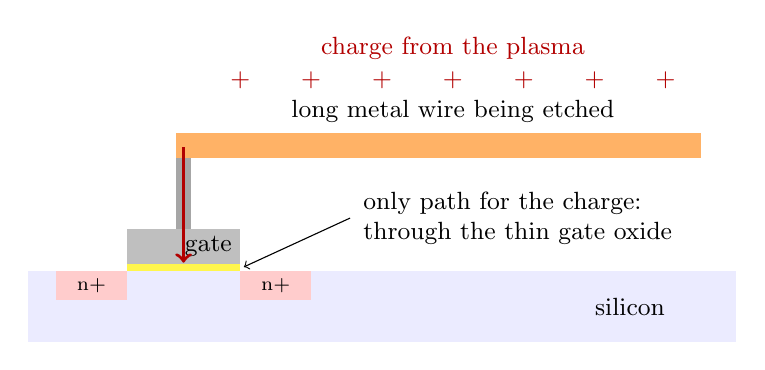
\begin{tikzpicture}[scale=0.9]
  \fill[blue!8] (0,0) rectangle (10,1); \node at (8.5,0.5) {\small silicon};
  \fill[red!20] (0.4,0.6) rectangle (1.4,1); \fill[red!20] (3.0,0.6) rectangle (4.0,1);
  \node[font=\scriptsize] at (0.9,0.8) {n+}; \node[font=\scriptsize] at (3.5,0.8) {n+};
  \fill[yellow!70] (1.4,1) rectangle (3.0,1.1);
  \fill[gray!50] (1.4,1.1) rectangle (3.0,1.6); \node[font=\small] at (2.55,1.35) {gate};
  \fill[gray!70] (2.1,1.6) rectangle (2.3,2.6);
  \fill[orange!60] (2.1,2.6) rectangle (9.5,2.95);
  \node[font=\small] at (6,3.25) {long metal wire being etched};
  \foreach \x in {3,4,...,9} \node[red!70!black,font=\small] at (\x,3.7) {$+$};
  \node[font=\small,red!70!black] at (6,4.15) {charge from the plasma};
  \draw[->,very thick,red!70!black] (2.2,2.75) -- (2.2,1.12);
  \node[font=\small,anchor=west,align=left] at (4.6,1.75) {only path for the charge:\\through the thin gate oxide};
  \draw[->] (4.55,1.75) -- (3.05,1.06);
\end{tikzpicture}
\caption{The antenna effect: a long wire connected only to a gate funnels plasma charge through the gate oxide.}
\label{fig:antenna}
\end{figure}

\paragraph{The antenna rule.} The danger depends on how much charge is collected compared with how much oxide area it is spread over. So the rule limits the \term{antenna ratio}:
\[
  \text{antenna ratio} = \frac{\text{area of metal connected to the gate (during that etch)}}{\text{area of the gate oxide it connects to}}.
\]
The factory gives a maximum ratio for each layer. Notice what each side means:
\begin{itemize}
  \item More metal (a longer wire) collects more charge: \textbf{worse}.
  \item More gate area spreads the charge over more oxide: \textbf{better}.
\end{itemize}

\begin{onoa}
The assessment asked, true or false: ``For the antenna rule, as long as the metal wire is safe, a small connected transistor is good.'' This is \textbf{false}. The wire is not ``safe'' or ``unsafe'' on its own; what matters is the \emph{ratio} of metal area to gate area. A \emph{smaller} gate means a \emph{larger} ratio, so a small connected transistor makes an antenna violation \emph{more} likely. A larger gate (or several gates) on the same wire is safer.
\end{onoa}

\paragraph{Fixing antenna violations.}
\begin{itemize}
  \item \textbf{Antenna diode}: add a small diode from the wire to the substrate near the gate. During etching it gives the charge a safe path to the silicon. In normal operation the diode is reverse biased, so it only adds a little leakage and capacitance (Chapter~\ref{ch:semis}).
  \item \textbf{Metal jumper (layer hopping)}: break the long wire and route part of it on a higher layer. While the lower layer is etched, the gate sees only a short piece of metal; by the time the higher layer is etched, the connection to the driver's diffusion is complete and the charge can drain.
  \item \textbf{Buffer insertion}: insert a buffer near the vulnerable gate, splitting the long wire into two nets, each with a smaller ratio.
  \item \textbf{Larger gate area}: a bigger receiving transistor lowers the ratio (at a cost in power and loading).
\end{itemize}

\section{Electromigration}

Electrons flowing through a wire collide with its metal atoms and, very slowly, push them along in the direction of electron flow. Over months and years this \term{electromigration} (EM) leaves \term{voids} where atoms have left (which can break the wire open) and \term{hillocks} where they pile up (which can short to a neighbor).

The median time to failure follows \term{Black's equation}:
\[
  \text{MTTF} = A\,J^{-n}\,e^{E_a/kT},
\]
where $J$ is the current density, $n$ is typically around 2, $E_a$ is an activation energy, and $T$ is absolute temperature. Two lessons: higher current density shortens life sharply, and higher temperature shortens it \emph{exponentially}.

Wires that carry steady current in one direction (power and ground) are most at risk; signal wires, whose current flows back and forth, are less so. Designers prevent EM failures by limiting current density: wider wires, more parallel wires, and multiple vias at every connection. Copper's better EM resistance was one reason it replaced aluminum.

\section{Latch-up}

A CMOS chip accidentally contains a parasitic structure that can short the supply to ground. Follow the layers from $\VDD$ to ground through a PMOS and a nearby NMOS: the PMOS's p+ source, the n-well, the p-type substrate, and the NMOS's n+ source. That is p-n-p-n, a four-layer device called a \term{thyristor} (or SCR), which behaves like two bipolar transistors feeding each other.

\begin{figure}[h]
\centering
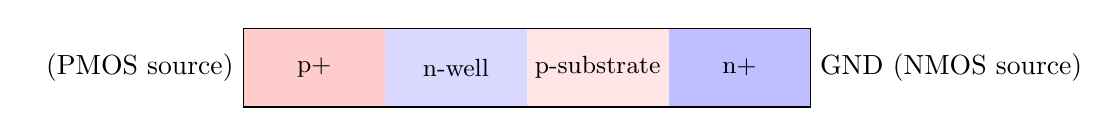
\begin{tikzpicture}
  \foreach \x/\lab/\col in {0/p+/red!20, 1.8/n-well/blue!15, 3.6/p-substrate/red!10, 5.4/n+/blue!25}
    { \fill[\col] (\x,0) rectangle (\x+1.8,1); \node at (\x+0.9,0.5) {\small \lab}; }
  \draw (0,0) rectangle (7.2,1);
  \node[left] at (0,0.5) {$\VDD$ (PMOS source)};
  \node[right] at (7.2,0.5) {GND (NMOS source)};
\end{tikzpicture}
\caption{The parasitic p-n-p-n path inside CMOS. Once triggered, it can latch into a low-resistance state between the supply and ground.}
\end{figure}

Normally this structure is off. But a disturbance that injects current into the well or substrate, such as a voltage spike on an input pin, an ESD event or a radiation strike, can turn both parasitic transistors on. Each then keeps the other on: the structure \emph{latches}, conducting heavily from $\VDD$ to ground until power is removed, often destroying the chip.

\paragraph{Prevention.} Keep the well and substrate firmly tied to their supplies with frequent \term{well taps} and \term{substrate taps} (low resistance there keeps the parasitic transistors from turning on); surround sensitive or I/O transistors with \term{guard rings}; keep NMOS and PMOS devices apart; or use processes that isolate transistors completely (such as silicon-on-insulator).

\section{Electrostatic discharge}

Walking across a carpet can charge your body to thousands of volts. Touching a chip's pin discharges that through the chip in nanoseconds. Gate oxides break down at only a few volts, so an unprotected input would be destroyed instantly. Every I/O pad therefore has \term{ESD protection}: diodes from the pad to $\VDD$ and to ground, plus clamp circuits between the supplies, which steer the discharge current around the core circuitry. ESD structures add capacitance to every pin, which is a challenge for very high-speed I/O.

\section{Aging and soft errors}

\paragraph{Wear-out.} Transistors degrade slowly under voltage and heat:
\begin{itemize}
  \item \term{NBTI} (negative bias temperature instability): PMOS thresholds rise over time while the transistor is on.
  \item \term{HCI} (hot-carrier injection): fast-moving carriers get trapped in the gate oxide, degrading the transistor.
  \item \term{TDDB} (time-dependent dielectric breakdown): the gate oxide eventually wears out under a strong electric field.
\end{itemize}
Designs include an \textbf{aging guardband} in their timing so they still work after years.

\paragraph{Soft errors.} A neutron from cosmic rays, or an alpha particle from trace radioactive impurities, can deposit enough charge to flip a bit in an SRAM cell or a flip-flop without damaging anything. These \term{soft errors} are handled with parity and error-correcting codes (Chapter~\ref{ch:memory}).

\section{Testing manufactured chips}

Factory testing looks for manufacturing defects, not design bugs. The standard model is the \term{stuck-at fault}: a node permanently stuck at 0 or 1. Scan chains (Chapter~\ref{ch:latch}) let testers load every flip-flop with a pattern, run one clock cycle, and read every result back out. Software (\term{ATPG}, automatic test pattern generation) finds a small set of patterns that detect nearly all possible stuck-at faults. Memories have built-in self-test (\term{BIST}) circuits that run test patterns on themselves.

\section{Summary}

\begin{itemize}
  \item Chips are printed layer by layer with photolithography; transistors first (FEOL), then wires (BEOL).
  \item Yield falls exponentially with die area ($Y = e^{-DA}$), motivating redundancy and chiplets.
  \item DRC checks shapes; LVS checks that the layout matches the netlist.
  \item Antenna effect: plasma charge on a wire connected only to a gate flows through the gate oxide. The rule limits metal area / gate area; a small gate is \emph{worse}. Fixes: diodes, layer jumpers, buffers, larger gates.
  \item Electromigration: current density and heat move metal atoms; MTTF $\propto J^{-n}e^{E_a/kT}$.
  \item Latch-up: a parasitic p-n-p-n thyristor shorts $\VDD$ to ground; prevented by taps and guard rings.
  \item ESD protection diodes guard every pin.
  \item Aging (NBTI, HCI, TDDB) needs guardbands; soft errors need ECC.
\end{itemize}

\section{Exercises}

\begin{enumerate}
  \item True or false: for the antenna rule, as long as the metal wire is safe, a small connected transistor is good. Explain.
  \item Give two ways to fix an antenna violation.
  \item With a defect density of 0.2 per cm$^2$, what is the yield of a 2\,cm$^2$ die?
  \item Does electromigration get better or worse at higher temperature?
  \item What causes latch-up, and name two ways to prevent it.
  \item What is the difference between DRC and LVS?
  \item Why do layout tools add dummy metal fill?
  \item What protects a chip's input pins from static electricity?
  \item Why does doubling a die's area more than double its cost per working die?
\end{enumerate}

\subsection*{Answers}
\begin{enumerate}
  \item False. The risk depends on the ratio of metal area to gate area. A smaller gate gives a larger ratio, so the charge collected by the wire is concentrated on less oxide: more likely to cause damage.
  \item Any two of: an antenna diode near the gate; breaking the wire and jumping to a higher metal layer; inserting a buffer near the gate; increasing the gate area.
  \item $e^{-0.4} \approx 67\%$.
  \item Worse; lifetime falls exponentially as temperature rises.
  \item A parasitic p-n-p-n structure (two coupled parasitic bipolar transistors) between the PMOS and NMOS can be triggered by injected current and then holds a low-resistance path from $\VDD$ to ground. Prevent it with frequent well and substrate taps, guard rings, spacing, or isolated processes such as SOI.
  \item DRC checks that layout shapes obey the factory's geometric rules. LVS checks that the circuit extracted from the layout matches the intended schematic or netlist.
  \item To make the metal density uniform so chemical-mechanical polishing produces flat layers.
  \item ESD protection: diodes from each pad to the supply and ground, plus supply clamps, that divert the discharge current.
  \item Fewer dies fit on each wafer, and the fraction of working dies falls (yield $e^{-DA}$ drops as $A$ grows), so both effects raise the cost of each good die.
\end{enumerate}
